\documentclass[11pt,a4paper]{article}

\usepackage[utf8]{inputenc}
\usepackage[T1]{fontenc}
\usepackage{amsmath,amssymb}
\usepackage{booktabs}
\usepackage{graphicx}
\usepackage[margin=2.5cm]{geometry}
\usepackage[colorlinks=true,linkcolor=blue,citecolor=blue,urlcolor=blue]{hyperref}

\graphicspath{{../analysis/results/cnn/}}

\newcommand{\code}[1]{\texttt{#1}}
\newcommand{\csitl}{CsI(Tl)}

\title{Three-dimensional position reconstruction in monolithic scintillating
crystals with a convolutional neural network:\\
\large millimetric localization of 511~keV photoelectric events from an
$8\times8$ SiPM light map}
\author{J.J.~G\'omez-Cadenas \and Claude (Anthropic)}
\date{July 15, 2026 \\[2mm] \small Version 0.1 --- CNN reconstruction note}

\begin{document}
\maketitle

\begin{abstract}
We reconstruct the three-dimensional position of 511~keV photoelectric
interactions in monolithic \csitl{} and BGO crystals ($48\times48$~mm$^2$,
two radiation lengths deep) from the light distribution recorded by an
$8\times8$ SiPM matrix, using a compact convolutional neural network trained on
the calibrated CryspLight simulation. On independent test samples the network
reaches a resolution of $1.21/1.24/1.11$~mm (RMS, $x/y/z$) in \csitl{} and
$0.84/0.84/0.92$~mm in BGO. The depth coordinate is reconstructed linearly over
the entire crystal, including the region where classical width-based estimation
is degenerate, and BGO attains the best resolution of the two crystals with one
quarter of the light --- the light-pattern geometry, rather than
photostatistics, sets the current limit. This note documents the dataset, the
network architecture and its motivation, the exact symmetry augmentation, the
classical and machine-learning reference estimators, and the results, in a
pedagogical style. A second study replaces the truth-based selection with the
one available to a real experiment --- an energy window of $\pm2\sigma$ around
511~keV at realistic energy resolution (FWHM 6\% for \csitl{}, 10\% for BGO)
--- so that Compton topologies enter the sample; the global resolution on that
mixture is $2.0/2.0/2.1$~mm (68\% quantile, $x/y/z$) with 27\% of events
beyond 5~mm for \csitl{}, and $1.1/1.1/1.3$~mm with 10\% beyond 5~mm for BGO.
The tail is identified with the soft-recoil Compton population, motivating a
two-site reconstruction as the next step.
\end{abstract}

\tableofcontents

%=====================================================================
\section{Introduction}

A monolithic scintillating crystal read out by a photosensor matrix is an
attractive alternative to a segmented detector: it preserves the full active
volume, simplifies assembly, and --- crucially --- encodes the interaction
position \emph{continuously} in the shape of the detected light distribution.
Recovering that position is a pattern-recognition problem: each event produces
an $8\times8$ image (the number of photoelectrons per SiPM), and the task is to
infer from it the three coordinates $(x, y, z)$ of the energy deposit. The
depth coordinate $z$ (depth of interaction, DOI) is the prize: it removes
parallax in tomographic applications and enables path-length corrections in
timing measurements, and it is the coordinate a segmented detector gives up.

This note documents the first reconstruction study of the CryspLight program:
a convolutional neural network (CNN) that regresses $(x, y, z)$ from the light
map, trained and evaluated on the calibrated end-to-end simulation (gamma
transport, scintillation, photon transport through the UNIFIED optical model on
the GPU, photodetection). The study is deliberately idealized, so that the
information content of the light map itself is measured cleanly: events are
restricted to single photoelectric interactions fully contained in the crystal,
and the photodetection efficiency is flat at $0.40$ for both crystals. Within
that scope the result is strong: millimetric resolution in all three
coordinates, in both \csitl{} and BGO.

%=====================================================================
\section{The dataset}
\label{sec:dataset}

\paragraph{Simulation campaigns.} Two campaigns of $5\times10^5$ gammas of
511~keV each (configurations \code{runs/gammas\_csitl\_500k.toml} and
\code{runs/gammas\_bgo\_500k.toml}) enter the crystal uniformly over the front
face and travel along $+z$; the SiPM matrix sits on the opposite face, at
$z = 37.2$~mm for \csitl{} and $z = 22.4$~mm for BGO (two radiation lengths in
each material). The per-event output carries the $8\times8$ photoelectron map,
the total photoelectron count, and the interaction truth: position, energy and
process of the first and second interaction, and the interaction type.

\paragraph{Selection.} The training sample consists of events with a single,
fully contained photoelectric interaction: interaction type
\code{int\_type} $= 0$ and deposited energy above $510.5$~keV. These are events
in which the full gamma energy converts at one point --- the cleanest possible
association between one light map and one true position. The selection yields
$86\,463$ events in \csitl{} and $190\,395$ in BGO (the photoelectric fraction
grows with the atomic number of the absorber), divided $70/15/15$ into
training, validation and test samples. The validation sample steers the
training; the test sample is opened once, for the numbers and figures reported
here.

\paragraph{Inputs.} The network receives two objects per event, chosen so that
each carries one kind of information:
\begin{itemize}
  \item \textbf{the shape}: the light map divided by its total photoelectron
    count. After this normalization the map is a probability distribution over
    the 64 SiPMs --- it says \emph{where} the light went, independently of how
    much there was. The position information lives here.
  \item \textbf{the scale}: the logarithm of the total photoelectron count,
    standardized to zero mean and unit variance on the training sample, and
    injected into the network separately (Section~\ref{sec:net}). For
    photoelectric events at fixed energy this scalar varies only through the
    collection efficiency; keeping it separate prepares the same architecture
    for variable-energy (Compton) events, where shape and scale genuinely
    decouple.
\end{itemize}

\paragraph{Targets.} The three coordinates are scaled linearly to the interval
$[-1, 1]$: $t = 2x/L - 1$ with $L$ the crystal dimension. The network then
learns three quantities of comparable magnitude, which balances the loss
across coordinates; predictions are mapped back to millimetres for every
number quoted in this note.

%=====================================================================
\section{A classical reference: Anger logic}
\label{sec:anger}

The classical estimator of the interaction position, in use since the original
scintillation camera, takes the first moments of the light distribution. With
$w_{ij}$ the photoelectron count of the SiPM centred at $(x_i, y_j)$,
\begin{equation}
  \hat{x} = \frac{\sum_{ij} w_{ij}\, x_i}{\sum_{ij} w_{ij}}, \qquad
  \hat{y} = \frac{\sum_{ij} w_{ij}\, y_j}{\sum_{ij} w_{ij}},
\end{equation}
and the depth is estimated from the second moment --- the RMS radius of the
map around its centroid --- through a calibration curve $z(r)$ fitted on
training events (a cubic polynomial here). The estimator is transparent and
requires no training beyond the one-dimensional $z(r)$ fit, and it defines the
scale against which any learned estimator should be judged.

Its physics limitations are equally transparent, and instructive. The centroid
is pulled toward the crystal centre for events near an edge, because the
reflected light re-enters the sum from one side only; the depth--width relation
is single-valued only where the direct-light spot dominates the map, while for
shallow events the reflected glow saturates the width (the effect is visible in
the DOI figure of the end-to-end note). Both features appear quantitatively in
the results of Section~\ref{sec:results}, where Anger logic provides the
baseline column.

%=====================================================================
\section{The network}
\label{sec:net}

\subsection{Design considerations}

The input is an image, and the appropriate tool is a convolutional network ---
the architectural family that began with LeNet and AlexNet and matured through
VGG (small $3\times3$ kernels stacked in depth) and ResNet (residual
connections and batch normalization). Those historical networks were sized for
photographs of $224\times224$ pixels; our image has $8\times8$ pixels, each of
which is precious. The design below keeps the modern ingredients --- small
kernels, batch normalization, residual blocks, global average pooling --- and
adapts the resolution ladder to the geometry: the map is processed at full
$8\times8$ resolution first, reduced once to $4\times4$, and only then
summarized.

\subsection{The ingredients, pedagogically}

\paragraph{Convolution.} A $3\times3$ convolution slides a learned $3\times3$
weight pattern across the map and outputs, at every position, the correlation
of the local neighbourhood with that pattern. One layer with 64 such patterns
(``channels'') turns the raw map into 64 feature maps --- one may learn to
respond to a local maximum, another to a left-to-right gradient, another to a
flat plateau. Two properties make convolutions ideal here: the \emph{same}
pattern detector is applied at every position (weight sharing), which matches
the physics --- a scintillation spot looks the same wherever it lands --- and
locality, which matches the fact that the direct-light spot is a compact
feature.

\paragraph{Batch normalization.} Each feature map is standardized (zero mean,
unit variance over the training batch) before the nonlinearity, then rescaled
by two learned parameters. This keeps every layer working in the regime where
gradients are informative and makes the optimization robust to the choice of
learning rate.

\paragraph{Residual blocks.} A residual block computes a small correction and
adds it to its input: $\mathrm{out} = \mathrm{in} + F(\mathrm{in})$, with $F$
two convolutional layers. The identity path guarantees that a deeper network
can always represent what a shallower one does (set $F = 0$), so depth becomes
a resource rather than a risk; in practice residual networks train faster and
to better optima.

\paragraph{Global average pooling.} After the convolutional stages each of the
128 final channels is averaged over its spatial extent, producing a
128-component descriptor of the whole map. This replaces the large
fully-connected layers of the early architectures, keeps the parameter count
small, and lets the convolutional features --- rather than a memorized pixel
layout --- carry the information.

\paragraph{Scalar fusion.} The standardized $\log$(photoelectron count) is
concatenated to the 128-component descriptor, and a small two-layer head maps
the combined vector to the three outputs. The head is linear in its last
layer: the network regresses coordinates, and the output is unconstrained.

\subsection{The architecture}

\begin{table}[htbp]
\centering
\begin{tabular}{llrr}
  \toprule
  stage & operation & output shape & parameters \\
  \midrule
  stem    & $3\times3$ conv + BN + ReLU            & $64\times8\times8$  & 4\,352 \\
  stage 1 & $2\times$ residual block (64 ch.)      & $64\times8\times8$  & 148\,480 \\
  descent & $3\times3$ conv, stride 2, + BN + ReLU & $128\times4\times4$ & 73\,984 \\
  stage 2 & $2\times$ residual block (128 ch.)     & $128\times4\times4$ & 591\,872 \\
  pooling & global average                          & $128$               & --- \\
  fusion  & concatenate $\log N_{\rm pe}$           & $129$               & --- \\
  head    & linear 128 + ReLU, linear 3            & $3$                 & 11\,843 \\
  \midrule
  total   &                                         &                     & 830\,531 \\
  \bottomrule
\end{tabular}
\caption{CryspNet layer inventory. The flat-pixel reference network (MLP,
Section~\ref{sec:baselines}) has 83\,459 parameters.}
\label{tab:arch}
\end{table}

Table~\ref{tab:arch} lists the network, called CryspNet
(\code{analysis/cnn/model.py}); it has $0.83\times10^6$ parameters, three
orders of magnitude below the classic photographic architectures, sized to the
information content of a 64-pixel image.

\subsection{Training}

The loss is the Huber function applied per coordinate in the normalized target
space: quadratic for residuals below one tenth of the half-length, linear
beyond, so that the rare pathological event steers the fit gently rather than
quadratically. Optimization uses AdamW (learning rate $10^{-3}$, weight decay
$10^{-4}$) with a cosine learning-rate schedule over 30 epochs and batches of
512 events; the model state with the best validation RMSE is kept. Training
runs on the Apple GPU through the PyTorch MPS backend and takes 51 minutes for
\csitl{} and 128 minutes for BGO (the larger sample), configurations
\code{analysis/cnn/runs/cnn\_\{csitl,bgo\}.toml}.

Figure~\ref{fig:conv} shows the convergence. The network reaches its
resolution plateau early: 97\% of the final \csitl{} performance by epoch 10,
and the BGO training settles by epoch 6; the reference perceptron descends
three times more slowly, a first appearance of the convolutional prior. Two
practical consequences follow. For exploratory work --- architecture variants,
new event classes --- a schedule of 10--15 epochs delivers essentially the
full resolution in a third of the time; and because the cosine schedule is
anchored to the \emph{planned} epoch count (the annealing completes whatever
the length), a shorter run configured through the \code{epochs} parameter is a
complete, properly scheduled training rather than an interrupted one.

\begin{figure}[htbp]
  \centering
  
\includegraphics[width=\textwidth]{cnn_csitl/convergence.png}
  \caption{\csitl{} training convergence: Huber loss on the training sample
  (left, logarithmic axis) and mean validation resolution (right) per epoch,
  for the network and the reference perceptron. The star marks the
  checkpoint retained for evaluation. The figure regenerates from
  \code{analysis/cnn/plot\_history.py}.}
  \label{fig:conv}
\end{figure}

%=====================================================================
\section{Exact symmetry augmentation}
\label{sec:d4}

The crystal is square in cross section and the SiPM grid shares its symmetry
axes, so the detector is invariant under the eight rigid transformations of
the square: the identity, three rotations, and four reflections (the dihedral
group $D_4$). Consequently, if a light map $M$ with true position $(x, y, z)$
is a possible event, then the rotated or reflected map with the correspondingly
transformed position is an \emph{equally probable} event --- a statement about
the geometry, exact to all orders, involving no approximation.

This yields a factor-eight enlargement of the training sample at zero
simulation cost: every training event enters under all eight transformations
(the depth coordinate is untouched). Beyond statistics, the augmentation
teaches the network the symmetry itself --- estimators trained this way treat
the four crystal quadrants identically by construction. The transformation
pairs (map operation, coordinate operation) are implemented in
\code{analysis/cnn/dataset.py}; a numerical self-test, run with
\code{python3 analysis/cnn/dataset.py}, places single bright pixels at known
positions and verifies that each of the eight operations maps the pixel centre
exactly onto the transformed target. The validation and test samples are used
untransformed.

%=====================================================================
\section{Reference estimators}
\label{sec:baselines}

Two references bracket the CNN. \textbf{Anger logic}
(Section~\ref{sec:anger}) represents the classical, training-free approach:
centroids for the transverse coordinates and the calibrated width--depth curve
for $z$. A \textbf{multilayer perceptron} (MLP) represents machine learning
without the convolutional structure: the 64 pixels are flattened to a vector,
concatenated with the same scalar, and passed through two hidden layers of 256
units. It is trained with identical data, augmentation, loss and schedule, so
the difference between MLP and CNN isolates the value of the convolutional
prior --- weight sharing and locality --- at this image size.

%=====================================================================
\section{Results}
\label{sec:results}

\begin{table}[htbp]
\centering
\begin{tabular}{llcccccc}
  \toprule
  & & \multicolumn{3}{c}{RMSE [mm]} & \multicolumn{3}{c}{68\% quantile [mm]} \\
  \cmidrule(lr){3-5}\cmidrule(lr){6-8}
  crystal & estimator & $x$ & $y$ & $z$ & $x$ & $y$ & $z$ \\
  \midrule
  \csitl{} (37.2 mm) & CryspNet & \textbf{1.21} & \textbf{1.24} & \textbf{1.11} & 0.96 & 0.99 & 0.89 \\
                     & MLP      & 1.49 & 1.48 & 1.35 & 1.25 & 1.26 & 1.21 \\
                     & Anger    & 11.71 & 11.79 & 8.64 & 13.51 & 13.79 & 9.13 \\
  \midrule
  BGO (22.4 mm)      & CryspNet & \textbf{0.84} & \textbf{0.84} & \textbf{0.92} & 0.74 & 0.75 & 0.84 \\
                     & MLP      & 0.97 & 0.98 & 1.12 & 0.89 & 0.90 & 1.05 \\
                     & Anger    & 11.19 & 11.17 & 5.77 & 12.97 & 12.97 & 6.02 \\
  \bottomrule
\end{tabular}
\caption{Position resolution on the test samples ($12\,970$ events for
\csitl{}, $28\,560$ for BGO): root-mean-square residual and 68\% quantile of
the absolute residual, per coordinate.}
\label{tab:results}
\end{table}

Table~\ref{tab:results} collects the resolutions;
Figures~\ref{fig:res-csitl}--\ref{fig:depth} document them. Three findings
stand out.

\paragraph{Millimetric localization in three dimensions.} The network resolves
the interaction position to $1.2$~mm transverse and $1.1$~mm in depth in
\csitl{}, and to $0.84$ and $0.92$~mm in BGO --- from an $8\times8$ image with
6~mm pixels. The residual distributions (Figures~\ref{fig:res-csitl}
and~\ref{fig:res-bgo}) are narrow, centred and symmetric for both learned
estimators, an order of magnitude inside the Anger reference in the transverse
coordinates.

\begin{figure}[htbp]
  \centering
  
\includegraphics[width=\textwidth]{cnn_csitl/residuals.png}
  \caption{\csitl{}: residual distributions of the three estimators in $x$
  (left), $y$ (centre) and $z$ (right) on the test sample.}
  \label{fig:res-csitl}
\end{figure}

\begin{figure}[htbp]
  \centering
  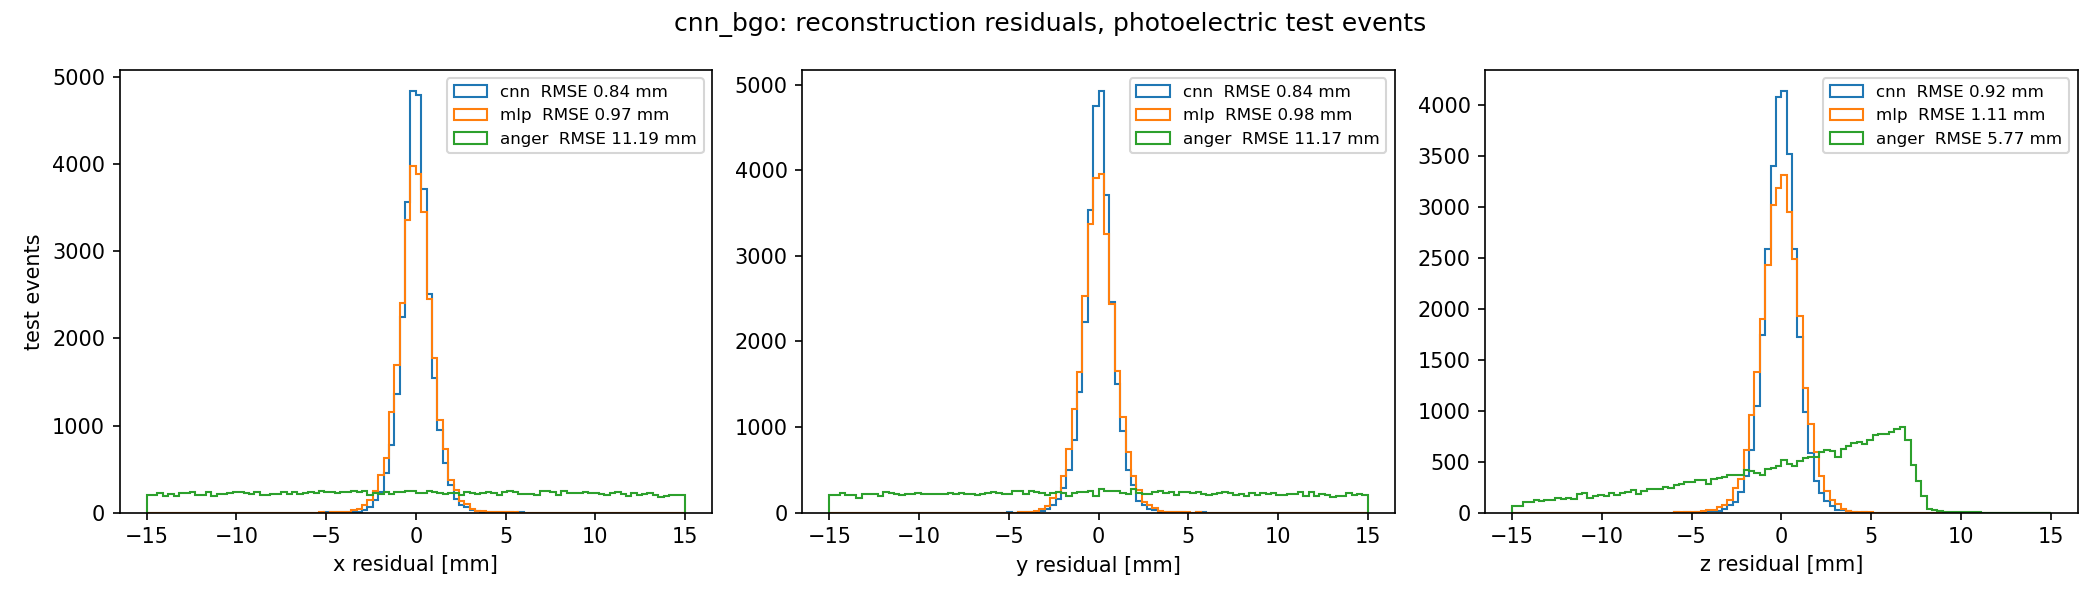
\includegraphics[width=\textwidth]{cnn_bgo/residuals.png}
  \caption{BGO: residual distributions of the three estimators in $x$ (left),
  $y$ (centre) and $z$ (right) on the test sample.}
  \label{fig:res-bgo}
\end{figure}

\paragraph{Depth reconstructed over the full crystal.} The resolution-versus-
depth curves (Figure~\ref{fig:rmsez}) show the network holding $0.3$--$1.7$~mm
in every coordinate across the entire depth range, and the true-versus-
predicted maps (Figure~\ref{fig:depth}) show a tight, linear diagonal from the
entrance face to the photosensor plane. The comparison with the width-based
classical estimator is the clearest physics statement of this study: the
width--depth calibration curve is informative only where the direct-light spot
dominates, whereas the network reads the full shape of the distribution ---
together with the collection-efficiency information carried by the
photoelectron count --- and extracts the depth everywhere.

\begin{figure}[htbp]
  \centering
  
\includegraphics[width=\textwidth]{cnn_csitl/rmse_vs_z.png}\\[2mm]
  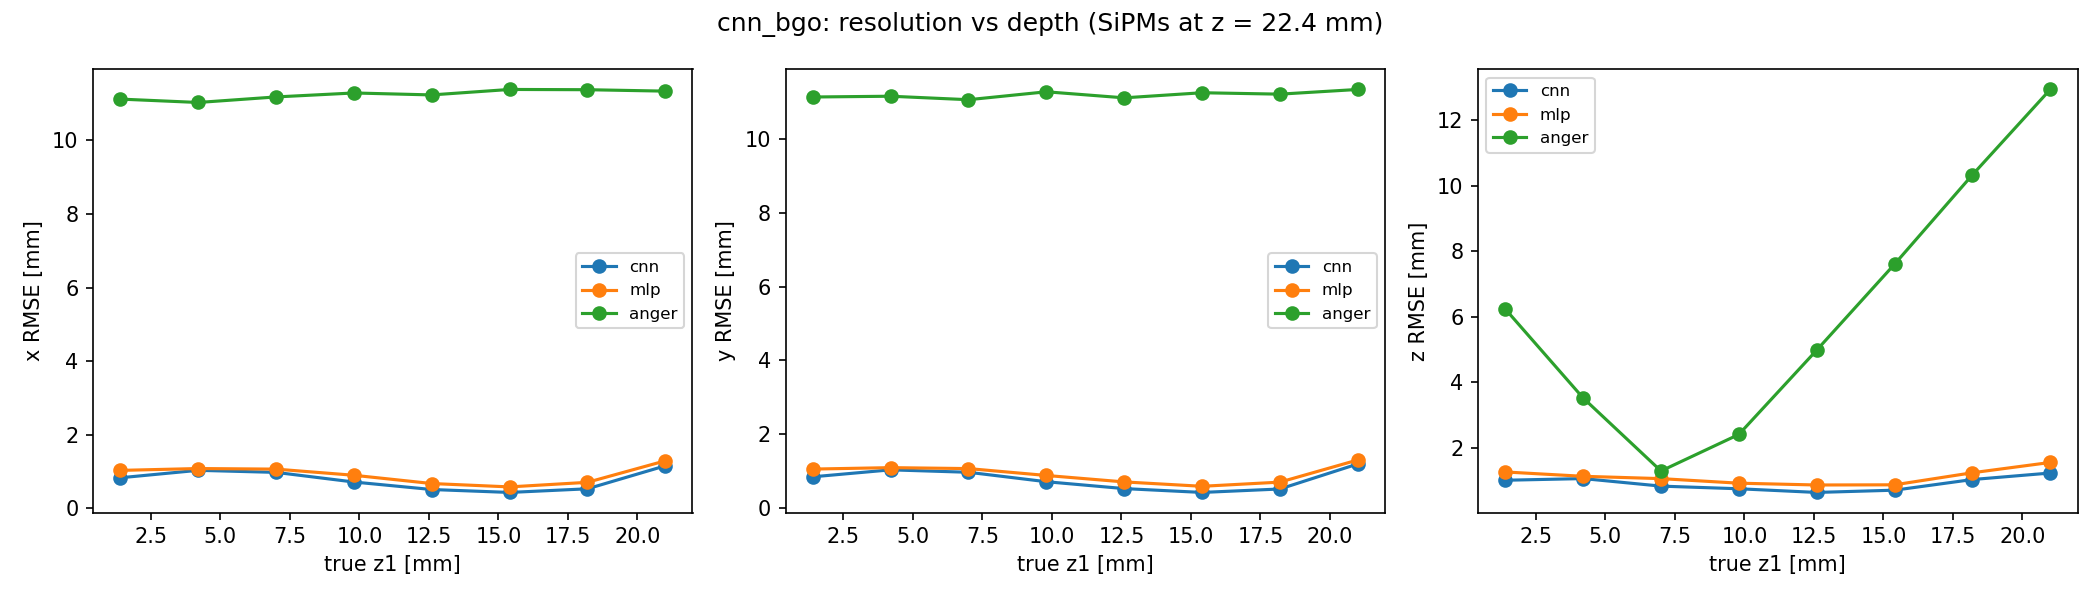
\includegraphics[width=\textwidth]{cnn_bgo/rmse_vs_z.png}
  \caption{Resolution versus true depth for \csitl{} (top) and BGO (bottom):
  $x$ (left), $y$ (centre) and $z$ (right). The SiPM plane sits at the right
  edge of each horizontal axis.}
  \label{fig:rmsez}
\end{figure}

\begin{figure}[htbp]
  \centering
  
\includegraphics[width=0.48\textwidth]{cnn_csitl/z_true_vs_pred.png}
  \hfill
  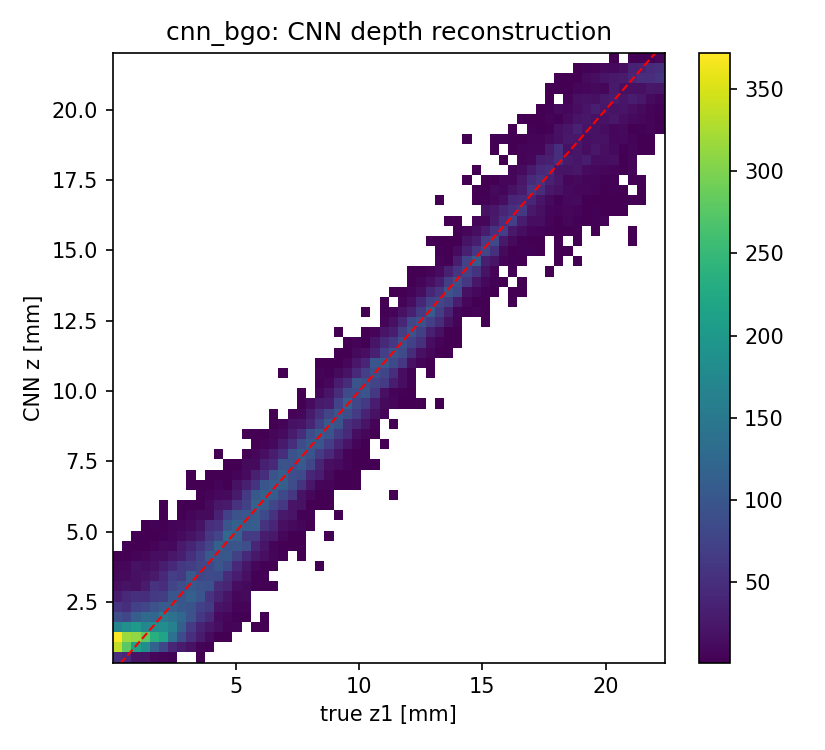
\includegraphics[width=0.48\textwidth]{cnn_bgo/z_true_vs_pred.png}
  \caption{Reconstructed versus true depth for the network, \csitl{} (left)
  and BGO (right); the dashed line marks perfect reconstruction.}
  \label{fig:depth}
\end{figure}

\paragraph{Geometry, rather than photostatistics, sets the limit.} BGO reaches
the best resolution of the two crystals while detecting one quarter of the
light ($\sim$2\,500 against $\sim$9\,800 photoelectrons at the photopeak). Its
shorter depth and higher refractive index produce light maps whose shape
varies more strongly with position, and the reconstruction rewards exactly
that. The comparison carries a design lesson for future geometries: optimizing
the position information of the light pattern can matter more than maximizing
the collected light.

\paragraph{The value of the convolutional prior.} The MLP, given identical
inputs, augmentation and training, lands within $20$--$25\%$ of the network in
every coordinate. At $8\times8$ pixels a fully-connected model can nearly
memorize the geometry, and the augmented sample is large; the convolutional
structure still wins consistently, and its advantage grows naturally with
richer inputs --- finer readout granularity, a second input channel, or the
multi-site topologies of Compton events.

%=====================================================================
\section{Reconstruction with realistic event selection}
\label{sec:window}

The study of Section~\ref{sec:results} selects events by their true
interaction type --- information available in simulation and nowhere else. A
real experiment selects on measured quantities, and the standard choice is an
energy window around the photopeak, whose purity is set by the energy
resolution of the detector. This section repeats the reconstruction under that
realistic selection.

\subsection{Selection and sample composition}

The measured energy is modelled as the true deposited energy smeared with the
full detector resolution: a Gaussian of fractional FWHM $6\%$ for \csitl{} and
$10\%$ for BGO at 511~keV, the width scaling as $\sqrt{E}$ below the peak.
Fully contained events deposit exactly 511~keV, so a window of
$511 \pm 2\sigma$ ($[485, 537]$~keV for \csitl{}, $[468, 554]$~keV for BGO)
retains $95.4\%$ of them by construction, together with a small leakage of
almost-contained events from below. The smear is applied with a fixed random
seed (configurations \code{analysis/cnn/runs/cnn\_\{csitl,bgo\}\_win.toml}),
making the selection reproducible.

The selected samples --- $243\,448$ events for \csitl{} and $360\,135$ for BGO
--- have the composition of the physical photopeak: for \csitl{}, $34\%$
single-site photoelectric events, $38\%$ with one Compton scatter, $28\%$ with
two or more; for BGO, $50\%$, $35\%$ and $15\%$. The reconstruction problem
changes character accordingly: for most events the light map is a superposition
of two or more energy-weighted sites, and the network, unchanged in
architecture and still regressing the \emph{first} interaction point, must
learn the mixture as a whole. Training uses the 15-epoch schedule
(Section~\ref{sec:net}), completing in 13 and 21 minutes.

\subsection{Global resolution}

Since the experiment has no means of separating the event classes, the
performance figure of the detector is the global one, over the full selected
sample. The residual distribution is now a narrow core under a long tail, and
a single RMS number would describe neither; the resolution is therefore quoted
as the pair (68\% quantile, fraction of events reconstructed farther than
5~mm from the true first interaction):

\begin{table}[htbp]
\centering
\begin{tabular}{lccccccc}
  \toprule
  & \multicolumn{3}{c}{68\% quantile [mm]} & \multicolumn{3}{c}{RMSE [mm]} &
  tail \\
  \cmidrule(lr){2-4}\cmidrule(lr){5-7}
  crystal & $x$ & $y$ & $z$ & $x$ & $y$ & $z$ & $d > 5$~mm \\
  \midrule
  \csitl{} & 2.02 & 2.03 & 2.08 & 3.19 & 3.24 & 4.16 & 26.8\% \\
  BGO      & 1.08 & 1.08 & 1.26 & 1.62 & 1.62 & 2.46 & 9.7\% \\
  \bottomrule
\end{tabular}
\caption{Global resolution of the network under the energy-window selection:
68\% quantile and RMSE of the residuals per coordinate, and the fraction of
events whose reconstructed point lies beyond 5~mm (3D distance) from the true
first interaction. Test samples of $36\,518$ (\csitl{}) and $54\,021$ (BGO)
events.}
\label{tab:window}
\end{table}

Millimetric localization survives contact with realistic selection: the
typical event is still reconstructed to $\sim$2~mm in \csitl{} and
$\sim$1.2~mm in BGO, in all three coordinates. BGO benefits doubly from its
photoelectric-rich composition and its shorter depth, and carries a tail three
times smaller.

\subsection{Anatomy of the tail}

Simulation truth, while unavailable for selection, remains the microscope for
\emph{evaluation}: breaking the residuals down by true interaction type
explains where the tail lives (Figure~\ref{fig:disttype} and
Table~\ref{tab:bytype}).

\begin{table}[htbp]
\centering
\begin{tabular}{llcccc}
  \toprule
  crystal & class & fraction & p68 $z$ [mm] & RMSE $z$ [mm] & $d > 5$~mm \\
  \midrule
  \csitl{} & photoelectric & 34\% & 1.07 & 1.46 & 2.0\% \\
           & one scatter   & 38\% & 2.33 & 4.20 & 29.8\% \\
           & two or more   & 28\% & 4.04 & 5.92 & 52.7\% \\
  \midrule
  BGO      & photoelectric & 50\% & 0.92 & 1.05 & 0.4\% \\
           & one scatter   & 35\% & 1.59 & 2.91 & 14.1\% \\
           & two or more   & 15\% & 2.82 & 4.17 & 31.4\% \\
  \bottomrule
\end{tabular}
\caption{Diagnostic breakdown of the window-sample residuals by true
interaction type (simulation truth used for evaluation only). The depth
coordinate is shown; the transverse coordinates behave alike.}
\label{tab:bytype}
\end{table}

\begin{figure}[htbp]
  \centering
  
\includegraphics[width=0.49\textwidth]{cnn_csitl_win/distance_by_type.png}
  \hfill
  
\includegraphics[width=0.49\textwidth]{cnn_bgo_win/distance_by_type.png}
  \caption{Distance between the reconstructed point and the true first
  interaction, by true interaction type, for \csitl{} (left) and BGO (right).
  The single-site class keeps a steeply falling distribution; the Compton
  classes add a tail extending to the inter-site distance scale.}
  \label{fig:disttype}
\end{figure}

Two findings frame the result. First, the single-site class survives the
mixture essentially intact: trained on a sample two-thirds of which is
multi-site, the network still reconstructs photoelectric events to
$1.28/1.30/1.46$~mm in \csitl{} and $0.90/0.88/1.05$~mm in BGO, within
$0.35$~mm of the truth-selected training of Section~\ref{sec:results} --- the
network distinguishes the topologies internally. Second, the tail is physics:
it is populated by Compton events whose first scatter deposits little energy,
so that the light map is dominated by the second site, centimetres away. For
that population a three-output network can only interpolate between the sites.
The remedy is expressiveness rather than capacity --- a network that predicts
\emph{both} interaction points, the subject of the next phase; its predicted
two-site separation will also provide an \emph{observable} event-quality flag,
turning the resolution--acceptance trade-off into an experimental choice. The
reference perceptron, trained once more for this comparison, trails the
network by $16$--$19\%$ globally and doubles its single-site tail; with the
convolutional advantage confirmed on the harder problem, subsequent studies
train the network alone.

%=====================================================================
\section{Outlook}

The idealized baseline is established. The extensions, in the order the
physics suggests them:

\begin{enumerate}
  \item \textbf{Two-site reconstruction.} A six-output network predicting both
    interaction points of the window sample, with the second target set
    coincident with the first for single-site events, addresses the Compton
    tail of Section~\ref{sec:window} directly; the predicted site separation
    doubles as an observable single-site discriminator.
  \item \textbf{Timing as a second channel.} The $8\times8$ matrix of
    first-photoelectron arrival times is recorded alongside the light map; the
    architecture accepts it as a second input channel by changing one number.
  \item \textbf{The response layer.} Intrinsic resolution and SiPM excess
    noise, applied as a post-processing smear, connect these results to
    measurable spectra.
  \item \textbf{Transverse-position diagnostics.} Resolution as a function of
    the distance to the crystal edge quantifies the boundary behaviour and
    guides possible readout optimizations.
\end{enumerate}

All results in this note regenerate from tracked configurations: the
simulation campaigns from \code{runs/gammas\_*\_500k.toml}, the trainings from
\code{analysis/cnn/runs/cnn\_*.toml}, and every figure from
\code{analysis/cnn/train.py}.

\end{document}
